\chapter{System fit and benefits}
\label{chap:fitsBenefits}
Content for this chapter will be provided after system integration and adoption
\section{Task-Technology Fit}
Task Technology Fit research introduced by Goodhue and Thompson in 1995 \cite{MES10} combines theories of job satisfaction and performance and applies them especially to situations in which utilization can be assumed. Further it argues that the effect of technology on performance cannot be measured independently from the task the technology is supposed to support\ref{fig:ttf}.
\begin{figure}[ht]
	\label{fig:ttf}
	\centering
	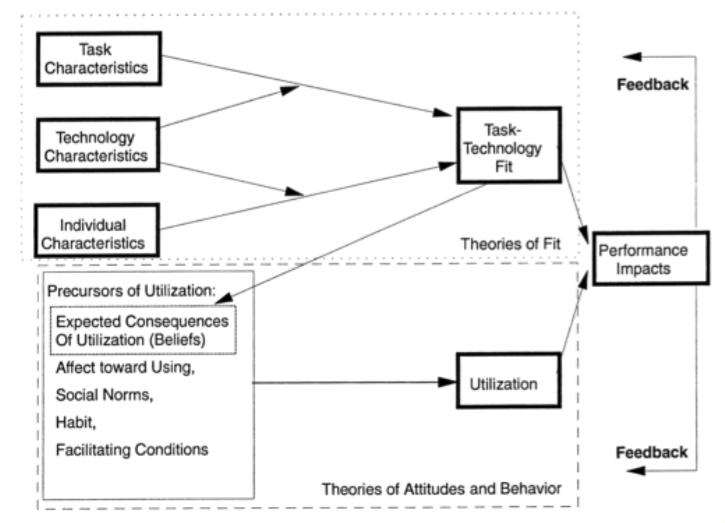
\includegraphics[width=\textwidth]{grafiken/ttf.png}
	\caption{Task-Technology Fit model\cite{MES10}}
\end{figure}

\subsection{Task characteristics}
\begin{itemize}
	\item Moving responsibility for test definition from developers to management staff
	\item Reduce time for bugs allocation and fixation
\end{itemize}


\subsection{Technology Characterisitcs}
\begin{itemize}
	\item Asynchronous software
	\item	Real-time software
\end{itemize}

\subsection{Individual Characterisitcs:}
\begin{itemize}
	\item  No developer background
\end{itemize}

\subsection{Task-Technology-Fit:}
\begin{itemize}
	\item Test Sheet - 
	\item Async node.js -
	\item Optimization for real-time execution - 
	\item Automatization of bug reporting process directly to the developer
\end{itemize}

\subsection{Utilization:}
\begin{itemize}
	\item Excel UX
	\item Simple conventions
\end{itemize}

\subsection{Performance Impact:}
Time measurements for tests generation
Time measurements for test executions and results representations

\section{Mistfits}
\subsection{Functionality missfits}
Functionality misfits occur, when the way processes are executed using the ES leads to reduced efficiency and effectivenes compared to pre-ES outcomes 

?

\subsection{Data misfits}
Data misfits occur, when data or data characteristics stored in or needed by the ES leads to data quality issues such as inaccuracy, inconsistent representation, inaccessibility, lack of timeliness or inappropriateness for users' context 

Example:
Expected: {“IBAN”: <String>}
Return: {“IBAN”: “loren ipsum”}

\subsection{Usability misfits}
Usability misfits occur, when the interactions with the ES required for task execution are cumbersome or confusing, i.e. requiring extra steps that add no value or introduce difficulty in entering or extracting information 

- Local store of code
- Local definitions of test

\subsection{Role misfits}
Role misfits occur, when the roles in the ES are inconcsistent with the skills available, create imbalances in the workload leading to bottlenecks and idle time, or generate mismatches between responsibility and authority 

Requires managements to store up-to-date code on their workstation

\subsection{Control misfits}
Control misfits occur, when the controls embedded in the ES provide too much control, inhibiting productivity, or too little control, leading to the inability to assess or monitor performance appropriately 

?

\subsection{Organizational culture}
Organizational culture misfits occur, when the ES requires ways of operating that countervene organizational norms 
?


\section{Benefits and affecting factors}
\paragraph{Organizational benefits} from system use from the perspective of senior management, is an overall measure of senior managemt's perception of the benefits from the IT-based application. Such benefits - which may be assessed either for the enterprise system investment overall, or from individual enterprise system projects - usually revolve around the software enabling faster, more accurate process coordination and execution, including links with business partners up and down the supply chain and greater accuracy of and visibility into organizational data, resulting in more tightly controlled organizational processes improved asset utilization and improved decision making.

\subsection{Short-term factor}
\paragraph{Functional Fit} is the extent to which the functional capabilities embedded and congigured within an enterprise system packge match the functionality that organization needs to operate effectively and efficiently. Saying that software has good functional fit is equivalent to saying that the processes supported by system are efficient and effiective for the organization and the software helps people in organization get their jobs done. It conceptualized as being delivered and measured project by project.
\paragraph{Oevercoming Organizational Inertia} is the extent to which members of the organization have been motivated to learn, use, and accept new system. During initial implementation and subsequent upgrade projects, considerable change-management effort, training, and support are needed to overcome organizational inertia.

\subsection{Long-term factor}
\paragraph{Integration} of information system is the unification of processes and/or data from multiple computer-based systems, not necessarily in the one organization.
\paragraph{Process optimization} is any attepmt to improve the efficiency and effectiveness of an organizations processes, ultimately in support of strategic goals.
\paragraph{Improved access to information} is any step take to increase the provision of timely, accurate, relevant information to key organizational decision making.
\paragraph{On-going major enterprise system improvement projects} is a measure of the number and extent of investment in major business improvement projects that an organization ha undertaken for improving and extending uts enterprise system. Major business projects are those that lead to changes in the way that work is done in the business.
\begin{table}[h]
	\begin{center}
		\begin{tabular}{| l | l |  }
			\hline
			\textbf{Cost reduction} & +  \\
			\hline
			\textbf{Cycle time reduction} & + \\
			\hline
			\textbf{Productivity improvement} & +  \\
			\hline
			\textbf{Quality improvement} & + \\
			\hline 
			\textbf{Customer Service improvement} & + \\
			\hline
		\end{tabular}
	\end{center}
	\caption{Operational Benefits of Test Sheets Use}
\end{table}

\begin{table}[h]
	\begin{center}
		\begin{tabular}{| l | l |  }
			\hline
			\textbf{Resource management} & +  \\
			\hline
			\textbf{Decision making and planning} & + \\
			\hline
			\textbf{Performance} & +  \\
			\hline
		\end{tabular}
	\end{center}
	\caption{Managerial Benefits of Test Sheets Use}
\end{table}

\begin{table}[h]
	\begin{center}
		\begin{tabular}{| l | l |  }
			\hline
			\textbf{Business growth} & +  \\
			\hline
			\textbf{Business alliance} & + \\
			\hline
			\textbf{Building business innovations} & +  \\
			\hline
			\textbf{Building cost leadership} & + \\
			\hline 
			\textbf{Product differentiation} & + \\
			\hline
			\textbf{External linkages} & + \\
			\hline
		\end{tabular}
	\end{center}
	\caption{Strategic Benefits of Test Sheets Use}
\end{table}

\begin{table}[h]
	\begin{center}
		\begin{tabular}{| l | l |  }
			\hline
			\textbf{Business flexibility for future challenges} & +  \\
			\hline
			\textbf{IT cost reduction} & + \\
			\hline
			\textbf{IT infrastructure capabilities} & +  \\
			\hline
		\end{tabular}
	\end{center}
	\caption{IT infrastructure Benefits of Test Sheets Use}
\end{table}

\begin{table}[h]
	\begin{center}
		\begin{tabular}{| l | l |  }
			\hline
			\textbf{Changing work patterns} & +  \\
			\hline
			\textbf{Facilitating organizational learning} & + \\
			\hline
			\textbf{Empowerment} & +  \\
			\hline
			\textbf{Building common vision} & + \\
			\hline
		\end{tabular}
	\end{center}
	\caption{Organizational Benefits of Test Sheets Use}
\end{table}


